% !TeX program = pdflatex
% !TeX root = main.tex
\documentclass[twocolumn]{article}
\usepackage[utf8]{inputenc}
\usepackage[T1]{fontenc}
\usepackage{lmodern}
\usepackage[spanish,es-nodecimaldot]{babel}
\usepackage[noieeebox]{ieeepes}
\usepackage{booktabs}
\usepackage{url}
\usepackage{graphicx}
\usepackage{amsmath,amssymb}
\usepackage{cite}
\usepackage{microtype}
\usepackage{float}

% Configuración para que Título, Autores, Resumen y Palabras clave aparezcan juntos a ancho completo (horizontal) en la primera página
\makeatletter
\newcommand{\resumen}[1]{\gdef\@resumentext{#1}}
\newcommand{\palabrasclave}[1]{\gdef\@palabrasclavetext{#1}}

% Desactivar caja flotante vacía inferior de ieeepes para evitar saltos de página indeseados
\let\@putbox\relax

\renewcommand\@putheader{%
  \twocolumn[%
    \begin{center}
      {\Large\textbf{\@title}\par}
      \vspace{0.6cm}
      {\large\textrm{\@author}\par}
      \vspace{0.6cm}
    \end{center}
    \ifdefined\@resumentext
      \begingroup
      \leftskip=0.3cm\rightskip=0.3cm
      \small
      \noindent\textbf{\textit{Resumen---}}\ignorespaces\@resumentext\par
      \ifdefined\@palabrasclavetext
        \vspace{0.6em}
        \noindent\textbf{\textit{Palabras clave---}}\ignorespaces\@palabrasclavetext\par
      \fi
      \endgroup
      \vspace{0.8cm}
    \fi
  ]
}
\makeatother

\title{Integraci\'on de Blockchain para la Trazabilidad y Auditor\'ia en el Entrenamiento Distribuido de Modelos de Inteligencia Artificial}

\author{David Piotr Znojek \\ Francisco A. Pujol L\'opez\\
Departamento de Tecnolog\'ia Inform\'atica y Computaci\'on\\
Escuela Polit\'ecnica Superior, Universidad de Alicante\\
Alicante, Espa\~na\\
\texttt{dpz6@alu.ua.es, fpujol@ua.es}}

\resumen{El entrenamiento distribuido mediante Aprendizaje Federado (\textit{Federated Learning}) permite preservar la privacidad de datos sensibles
pero carece intr\'insecamente de mecanismos para auditar la legitimidad de las contribuciones de los participantes, exponiendo al sistema a ataques de
envenenamiento (\textit{model poisoning}) con consecuencias cr\'iticas en sectores como el de los veh\'iculos aut\'onomos. En este art\'iculo se presenta
y eval\'ua una arquitectura h\'ibrida que integra una red Blockchain permisionada basada en Hyperledger Besu y consenso IBFT 2.0 con el framework Flower y
almacenamiento distribuido fuera de cadena mediante IPFS. Se dise\~na un contrato inteligente en Solidity que implementa un protocolo de doble verificaci\'on
cruzada entre clientes y servidor agregador utilizando compromisos criptogr\'aficos SHA-256 de los pesos neuronales. La viabilidad del marco se valida emp\'iricamente
sobre un banco de pruebas distribuido entrenando un clasificador convolucional de se\~nales y eventos viales a lo largo de 30 rondas bajo cinco configuraciones experimentales.
Los resultados cuantitativos demuestran que la capa de trazabilidad a\~nade una sobrecarga temporal reducida de entre el 6,2\% (5,22~s en entorno local) y el 10,9\% (7,03~s en entorno distribuido),
manteniendo un consumo de gas estrictamente constante ($\mathcal{O}(1)$) y escalando con m\'inima variaci\'on de latencia al aumentar de 4 a 7 nodos validadores.
Esta investigaci\'on confirma que el coste de incorporar inmutabilidad y no repudio resulta plenamente asumible frente a las garant\'ias de auditor\'ia obtenidas.}

\palabrasclave{Aprendizaje Federado, Blockchain, Hyperledger Besu, Trazabilidad, Consenso IBFT 2.0, IPFS, Auditor\'ia Criptogr\'afica.}

\date{}

\begin{document}
\maketitle

% !TeX root = ../main.tex
\section{Introducción}
\label{sec:introduccion}

El auge de la Inteligencia Artificial (IA) y del Aprendizaje Automático (\textit{Machine Learning}, ML) ha transformado sectores críticos como la salud, las finanzas y la conducción autónoma. No obstante, el entrenamiento de modelos de gran capacidad requiere volúmenes masivos de datos, frecuentemente sensibles o confidenciales (geolocalización, hábitos de consumo o registros biométricos). En los paradigmas tradicionales centralizados, la recopilación de información en un único repositorio introduce graves riesgos de privacidad, problemas de cumplimiento normativo (como el RGPD) y cuellos de botella computacionales y energéticos.

El Aprendizaje Federado (\textit{Federated Learning}, FL)~\cite{mcmahan2017federated} surgió como una alternativa descentralizada en la que múltiples nodos o clientes entrenan copias locales del modelo con sus propios datos privados, transmitiendo a un servidor central únicamente los parámetros o gradientes actualizados. Aunque FL solventa en gran medida la fuga de datos crudos, introduce una vulnerabilidad estructural: la falta de confianza intrínseca entre los participantes. En un entorno distribuido no supervisado, actores maliciosos o nodos comprometidos pueden ejecutar ataques de envenenamiento (\textit{data poisoning} o \textit{model poisoning}) inyectando pesos manipulados. Por ejemplo, en el contexto de los Vehículos Conectados y Autónomos (CAV), una pequeña alteración coordinada en los pesos podría inducir al modelo global a no clasificar correctamente una señal de tráfico crítica (como un STOP), con consecuencias potencialmente fatales.

Para mitigar este riesgo, la tecnología \textit{Blockchain} ofrece una solución idónea como registro contable inmutable, descentralizado y verificable~\cite{nakamoto2008bitcoin, zheng2018blockchain}. Al integrar Blockchain en un flujo de entrenamiento distribuido, cada actualización de parámetros, ronda de agregación e identidad de los clientes queda registrada criptográficamente mediante contratos inteligentes (\textit{smart contracts}), habilitando la trazabilidad absoluta y la no repudiación de las contribuciones.

Sin embargo, esta convergencia plantea un compromiso técnico fundamental: el dilema entre \textbf{seguridad y rendimiento}. Mientras que la Blockchain garantiza inmutabilidad y consenso bizantino, introduce una sobrecarga inevitable de latencia de red, tiempo de confirmación de transacciones y consumo de recursos. En aplicaciones de misión crítica o en tiempo cuasi-real, resulta imperativo responder a la siguiente pregunta: \textit{¿cuánta latencia y coste computacional estamos dispuestos a asumir a cambio de un entrenamiento auditable y más resistente a manipulaciones?}

\subsection{Motivación y Trabajos Previos}
Este trabajo se fundamenta y amplía dos líneas de investigación desarrolladas en la Universidad de Alicante:
\begin{enumerate}
    \item \textbf{Verificación de eventos vehiculares en tiempo real}~\cite{pujol2024blockchain}: demostró la viabilidad de una red privada Hyperledger Besu con consenso IBFT 2.0 para registrar alertas de tráfico con latencias de 0,32 a 0,82 segundos, mejorando el tiempo de respuesta humano.
    \item \textbf{Framework FL-Blockchain}~\cite{cloudlabaia_flblockchain}: planteó conceptualmente el uso de contratos inteligentes para registrar los \textit{hashes} criptográficos de los pesos de entrenamiento en cada ronda federada.
\end{enumerate}

La presente investigación valida, formaliza e implementa experimentalmente la convergencia de ambas propuestas en un banco de pruebas real, evaluando tanto la integridad como el impacto en el rendimiento temporal.

\subsection{Contribuciones Principales}
Las contribuciones de este artículo se resumen en los siguientes puntos:
\begin{itemize}
    \item \textbf{Diseño de una arquitectura híbrida}: Se formula un marco integral que acopla una red permisionada basada en Hyperledger Besu con el framework de aprendizaje federado Flower~\cite{beutel2020flower} y un sistema de almacenamiento distribuido direccionable por contenido (IPFS).
    \item \textbf{Trazabilidad e integridad mediante Smart Contracts}: Se diseña un contrato inteligente en Solidity que orquesta la verificación cruzada de modelos mediante resúmenes SHA-256, registrando de forma inalterable las contribuciones de cada cliente y el modelo global consolidado por ronda.
    \item \textbf{Evaluación empírica y mitigación de ataques adversariales}: Se somete la infraestructura a vectores de ataque deliberados de inyección de pesos corruptos (tanto en servidor comprometido como en clientes envenenadores), validando la capacidad del protocolo de doble verificación para detectar y neutralizar el fraude con una efectividad del 100\% y tiempos de reacción inferiores a $0{,}1$~segundos.
    \item \textbf{Evaluación cuantitativa de la infraestructura}: Se despliega un clasificador convolucional de tráfico con el propósito de emplear la estructura de aprendizaje federado como banco de pruebas experimental para extraer métricas cuantitativas reproducibles (sobrecoste temporal, consumo de gas y escalabilidad de validadores), delimitando la optimización fina del modelo como trabajo futuro.
    \item \textbf{Análisis de viabilidad operativa}: Se responde analíticamente al dilema latencia-seguridad, delimitando los escenarios en los que la sobrecarga del registro en cadena resulta plenamente asumible frente a esquemas no auditables.
\end{itemize}

\subsection{Estructura del Artículo}
El resto del manuscrito se estructura de la siguiente manera: la Sección~\ref{sec:estado_arte} expone el estado del arte y fundamentos teóricos de Blockchain y Aprendizaje Federado. La Sección~\ref{sec:arquitectura} detalla la arquitectura propuesta y el diseño del contrato inteligente. La Sección~\ref{sec:implementacion} describe el banco de pruebas experimental y el dataset empleado. La Sección~\ref{sec:evaluacion} presenta y discute los resultados de rendimiento y seguridad. Finalmente, la Sección~\ref{sec:conclusiones} resume las conclusiones y líneas futuras.


% !TeX root = ../main.tex
\section{Fundamentos Teóricos y Trabajos Relacionados}
\label{sec:estado_arte}

La arquitectura propuesta converge tres pilares tecnológicos: registros distribuidos permisionados con consenso BFT, almacenamiento direccionable por contenido y aprendizaje federado. A continuación se sintetizan sus fundamentos teóricos y las limitaciones detectadas en la literatura.

\subsection{Blockchain Permisionada y Consenso IBFT 2.0}
Una cadena de bloques es una estructura de datos inmutable y distribuida en la que las transacciones se agrupan en bloques encadenados mediante funciones hash criptográficas resistentes a colisiones (como SHA-256)~\cite{nist2015sha, zheng2018blockchain}. Frente a las redes públicas (\textit{permissionless}) como Bitcoin o Ethereum Mainnet, penalizadas por altas latencias y costes económicos de transacción, los consorcios industriales adoptan redes permisionadas basadas en la Máquina Virtual de Ethereum (EVM)~\cite{buterin2014ethereum}, tales como Hyperledger Besu~\cite{besu_docs}.
\\

En estos entornos, los mecanismos basados en consumo de recursos (PoW) o capital (PoS) se sustituyen por algoritmos de tolerancia a fallos bizantinos. El protocolo \textbf{IBFT 2.0} (\textit{Istanbul Byzantine Fault Tolerant})~\cite{moniz2020istanbul} estructura el consenso en torno a un conjunto predefinido de validadores que alternan el rol de proponente mediante un esquema rotatorio (\textit{round-robin}). Un bloque solo se anexa a la cadena tras una votación en tres fases (pre-prepare, prepare, commit) firmada por una supermayoría de al menos dos tercios:
\begin{equation}
n \ge 3f + 1
\end{equation}
donde $n$ denota el número total de nodos validadores y $f$ el número máximo de participantes defectuosos o bizantinos tolerables. 
\\

IBFT 2.0 ofrece una propiedad determinante frente a otros consensos: la \textbf{finalidad determinista inmediata}. Al carecer de bifurcaciones probabilísticas (\textit{forks}), una vez que una ronda de entrenamiento o contribución se sella en un bloque, es irrefutable y permanente. Asimismo, aunque el precio del gas (\textit{gas price}) se configure en cero para anular tarifas monetarias, el cómputo de \textit{gas used}~\cite{ethereum_gas} se mantiene como métrica objetiva del coste de cómputo y almacenamiento impuesto a la red.

\subsection{Almacenamiento Distribuido Off-Chain (IPFS)}
El almacenamiento directo de redes neuronales profundas en una Blockchain es inviable debido al tamaño de los pesos (decenas o cientos de megabytes), lo cual provocaría una saturación crítica del estado de la EVM (\textit{state bloat}) y un consumo prohibitivo de gas.
\\

Para superar este cuello de botella, se implementa el paradigma de \textbf{almacenamiento fuera de cadena con compromiso dentro de cadena} (\textit{off-chain storage with on-chain commitment}) utilizando el Sistema de Archivos Interplanetario (IPFS)~\cite{benet2014ipfs}. IPFS opera sobre una topología P2P basada en direccionamiento por contenido (\textit{content addressing}): cada archivo se identifica de forma unívoca mediante un \textit{Content Identifier} (CID), obtenido a partir del hash criptográfico de su contenido. Al registrar únicamente el CID y el hash SHA-256 en el contrato inteligente, se asegura que cualquier descarga posterior sea verificada bit a bit contra el registro inmutable, garantizando deduplicación, disponibilidad y verificación formal de integridad con coste computacional on-chain mínimo.

\subsection{Aprendizaje Federado y Algoritmo FedAvg}
El Aprendizaje Federado (FL)~\cite{mcmahan2017federated} resuelve la preservación de la privacidad de datos crudos al desacoplar el entrenamiento local de la agregación global. Entre los algoritmos de consenso federado, \textbf{FedAvg} (\textit{Federated Averaging}) representa el estándar fundacional. En cada ronda de comunicación $t$, el servidor distribuye el vector de pesos global actual $w^{(t)}$ a un subconjunto de $K$ clientes seleccionados. Cada cliente entrena el modelo sobre su partición local $\mathcal{D}_k$ minimizando una función de pérdida, obteniendo los parámetros locales $w_k^{(t)}$. El servidor calcula el nuevo modelo global consolidado como la media ponderada del volumen de muestras locales $n_k$:
\begin{equation}
w^{(t+1)} = \sum_{k=1}^{K} \frac{n_k}{n} \, w_k^{(t)}, \quad \text{donde } n = \sum_{k=1}^{K} n_k
\end{equation}

El marco de referencia \textbf{Flower}~\cite{beutel2020flower} proporciona una infraestructura desacoplada y eficiente para orquestar este flujo mediante llamadas a procedimientos remotos bidireccionales sobre gRPC.

\subsection{Vulnerabilidades en FL y Trabajos Relacionados}
A pesar de sus ventajas de privacidad, los sistemas FL tradicionales sufren de severas vulnerabilidades de seguridad:
\begin{enumerate}
    \item \textbf{Servidor central como punto único de fallo y confianza}: No existe salvaguarda para verificar si el servidor manipuló la ponderación de FedAvg o si inyectó sesgos maliciosos en $w^{(t+1)}$.
    \item \textbf{Ataques de envenenamiento y falta de trazabilidad}: Nodos malintencionados pueden realizar \textit{model poisoning} o inyectar puertas traseras (\textit{backdoors}). Sin un historial no repudiable de identidades y hashes, resulta imposible deslindar qué participante contaminó el modelo global.
\end{enumerate}

Diversas aproximaciones en la literatura han explorado la hibridación de Blockchain y FL. No obstante, gran parte de los trabajos teóricos sufren de problemas de escalabilidad al pretender ejecutar la agregación matemática completa dentro de la EVM o depender de redes públicas costosas. En el dominio de los sistemas de transporte inteligentes (ITS), Pujol et al.~\cite{pujol2024blockchain} demostraron que Hyperledger Besu con IBFT 2.0 ofrece latencias subsegundo viables para la cooperación vehicular, y CloudLab-AIA~\cite{cloudlabaia_flblockchain} conceptualizó el registro de hashes de modelos. Este artículo capitaliza dichas investigaciones previas, materializando una arquitectura verificada de extremo a extremo que cuantifica exhaustivamente el balance entre coste temporal y auditabilidad criptográfica.


% !TeX root = ../main.tex
\section{Arquitectura del Sistema Propuesto}
\label{sec:arquitectura}

Para dotar al aprendizaje federado de trazabilidad y resistencia frente a comportamientos bizantinos, se propone una arquitectura híbrida desacoplada en tres planos operacionales: el plano de computación federada (Flower), el plano de almacenamiento direccionable fuera de cadena (IPFS) y el plano de consenso e inmutabilidad dentro de cadena (Hyperledger Besu). La Figura~\ref{fig:arq_sistema} ilustra la interacción integral entre estos componentes.

\begin{figure*}[t]
    \centering
    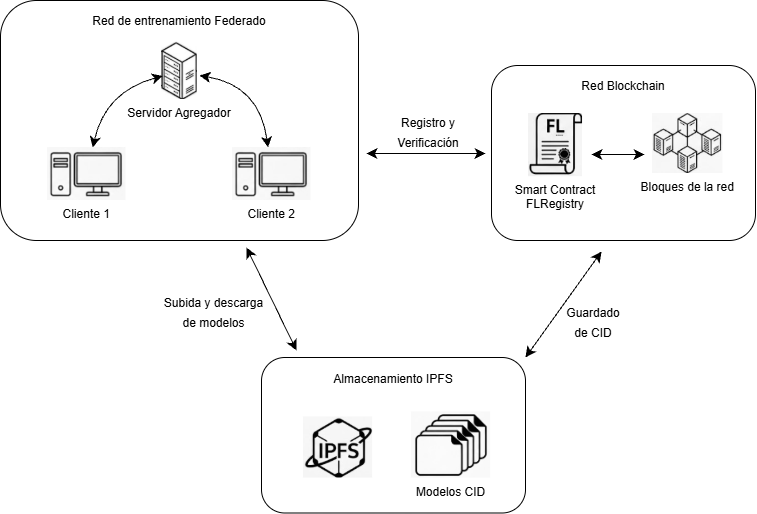
\includegraphics[width=0.88\textwidth]{figuras/ArqSistema.png}
    \caption{Arquitectura general del sistema híbrido: desacoplamiento entre el cómputo federado (Flower), el almacenamiento de pesos fuera de cadena (IPFS) y el registro inmutable de trazabilidad (Hyperledger Besu con IBFT 2.0).}
    \label{fig:arq_sistema}
\end{figure*}

\subsection{Diseño del Smart Contract: FLRegistry}
El componente de gobernanza y auditoría lógica se implementa mediante el contrato inteligente \texttt{FLRegistry}, codificado en Solidity (versión \texttt{0.8.10}). Su misión es registrar un historial criptográfico determinista de cada ronda sin albergar matrices numéricas masivas on-chain.
\\

\subsubsection{Estructuras de datos y persistencia}
La entidad nuclear del contrato es la estructura \texttt{ModelRound}, definida como:
\begin{verbatim}
struct ModelRound {
    uint256 roundNum;
    string modelHash;
    address author;
    uint256 timestamp;
}
\end{verbatim}
donde \texttt{roundNum} indexa la iteración federada, \texttt{modelHash} almacena el CID o digest SHA-256 del artefacto del modelo, \texttt{author} guarda la dirección pública Ethereum del emisor (\texttt{msg.sender}) y \texttt{timestamp} captura la marca temporal del bloque validado.
\\

El estado del contrato se organiza mediante dos tablas hash (\textit{mappings}) complementarias:
\begin{itemize}
    \item \texttt{mapping(uint256 => ModelRound) public \\ history}: almacena de forma secuencial los modelos globales agregados por el servidor al término de cada ronda $t$.
    \item \texttt{mapping(uint256 => mapping(address => \\ ModelRound)) public clientHistory}: indexa las contribuciones locales individuales de cada cliente en cada ronda, posibilitando la auditoría forense granular de las participaciones.
\end{itemize}

Adicionalmente, se mantienen los punteros de estado \texttt{latestRound} y el indicador booleano \texttt{hasModel} para optimizar lecturas directas $\mathcal{O}(1)$ sin requerir iteraciones sobre el almacenamiento persistente.
\\

\subsubsection{Primitivas de escritura y autenticación}
El contrato expone dos métodos transaccionales que alteran el estado y emiten el evento desacoplado \texttt{ModelUpdated}:
\begin{itemize}
    \item \texttt{updateModel(uint256 round, string memory hash)}: Invocado operacionalmente por el servidor tras converger el algoritmo de agregación. A nivel de diseño del banco de pruebas, la función se implementa con visibilidad pública para desacoplar el contrato de dependencias estáticas de despliegue; no obstante, la EVM registra de forma inmutable la dirección emisora en el campo \texttt{author} (\texttt{msg.sender}). Esto permite a los clientes verificar criptográficamente frente a la clave pública autorizada del servidor que el modelo global sellado proviene legítimamente del agregador del consorcio.
\end{itemize}

\subsubsection{Primitivas de lectura y verificación}
Para no sobrecargar la red con costes de ejecución, las consultas de verificación se implementan como funciones \texttt{view}, las cuales se resuelven localmente en el nodo RPC sin consumir gas:
\begin{itemize}
    \item \texttt{getLastModel()}: Permite a cualquier cliente recuperar el CID del último modelo global consolidado y su marca de tiempo.
    \item \texttt{getClientModel(uint256 round, address client)}: Permite al servidor y a auditores externos cotejar el CID reportado por un cliente frente a su registro on-chain firmado.
\end{itemize}

\subsection{Flujo Operacional y Doble Verificación Cruzada}
El ciclo de vida del entrenamiento federado se estructura en una fase de inicialización única seguida de un protocolo iterativo con verificación bidireccional estricta, como se resume a continuación:
\\

\subsubsection{Fase 0: Arranque y Modelo Base (Ronda 0)}
Antes de iniciar la concurrencia:
\begin{enumerate}
    \item Se inicializa la red Besu con consenso IBFT 2.0 y el daemon IPFS.
    \item Se despliega \texttt{FLRegistry} registrando su dirección y ABI en un descriptor JSON distribuido.
    \item El servidor instancia los pesos iniciales $w^{(0)}$, los serializa y los almacena en IPFS, recibiendo un CID inicial $\text{CID}_0$.
    \item El servidor ejecuta \texttt{updateModel(0, }$\text{CID}_0$\texttt{)}, fijando el punto de partida auditable para todos los participantes. \\
\end{enumerate}

\subsubsection{Fase 1: Verificación Descendente (Cliente protege frente a Servidor)}
Al recibir la señal de inicio de ronda junto con los pesos candidatos $w_{cand}^{(t)}$ vía gRPC (Figura~\ref{fig:flujo_cliente_verif}):
\begin{enumerate}
    \item El cliente consulta la Blockchain invocando \texttt{getLastModel()} y obtiene el $\text{CID}_{reg}^{(t-1)}$ oficial.
    \item El cliente descarga el modelo referenciado desde IPFS y realiza una verificación bit a bit tensor por tensor frente a $w_{cand}^{(t)}$.
    \item Si se detecta cualquier discrepancia entre los pesos entregados y el compromiso sellado en la cadena, el cliente \textbf{aborta el entrenamiento inmediatamente}, neutralizando ataques donde un servidor comprometido intente inyectar modelos sesgados selectivamente a clientes concretos.
\end{enumerate}

\begin{figure}[H]
    \centering
    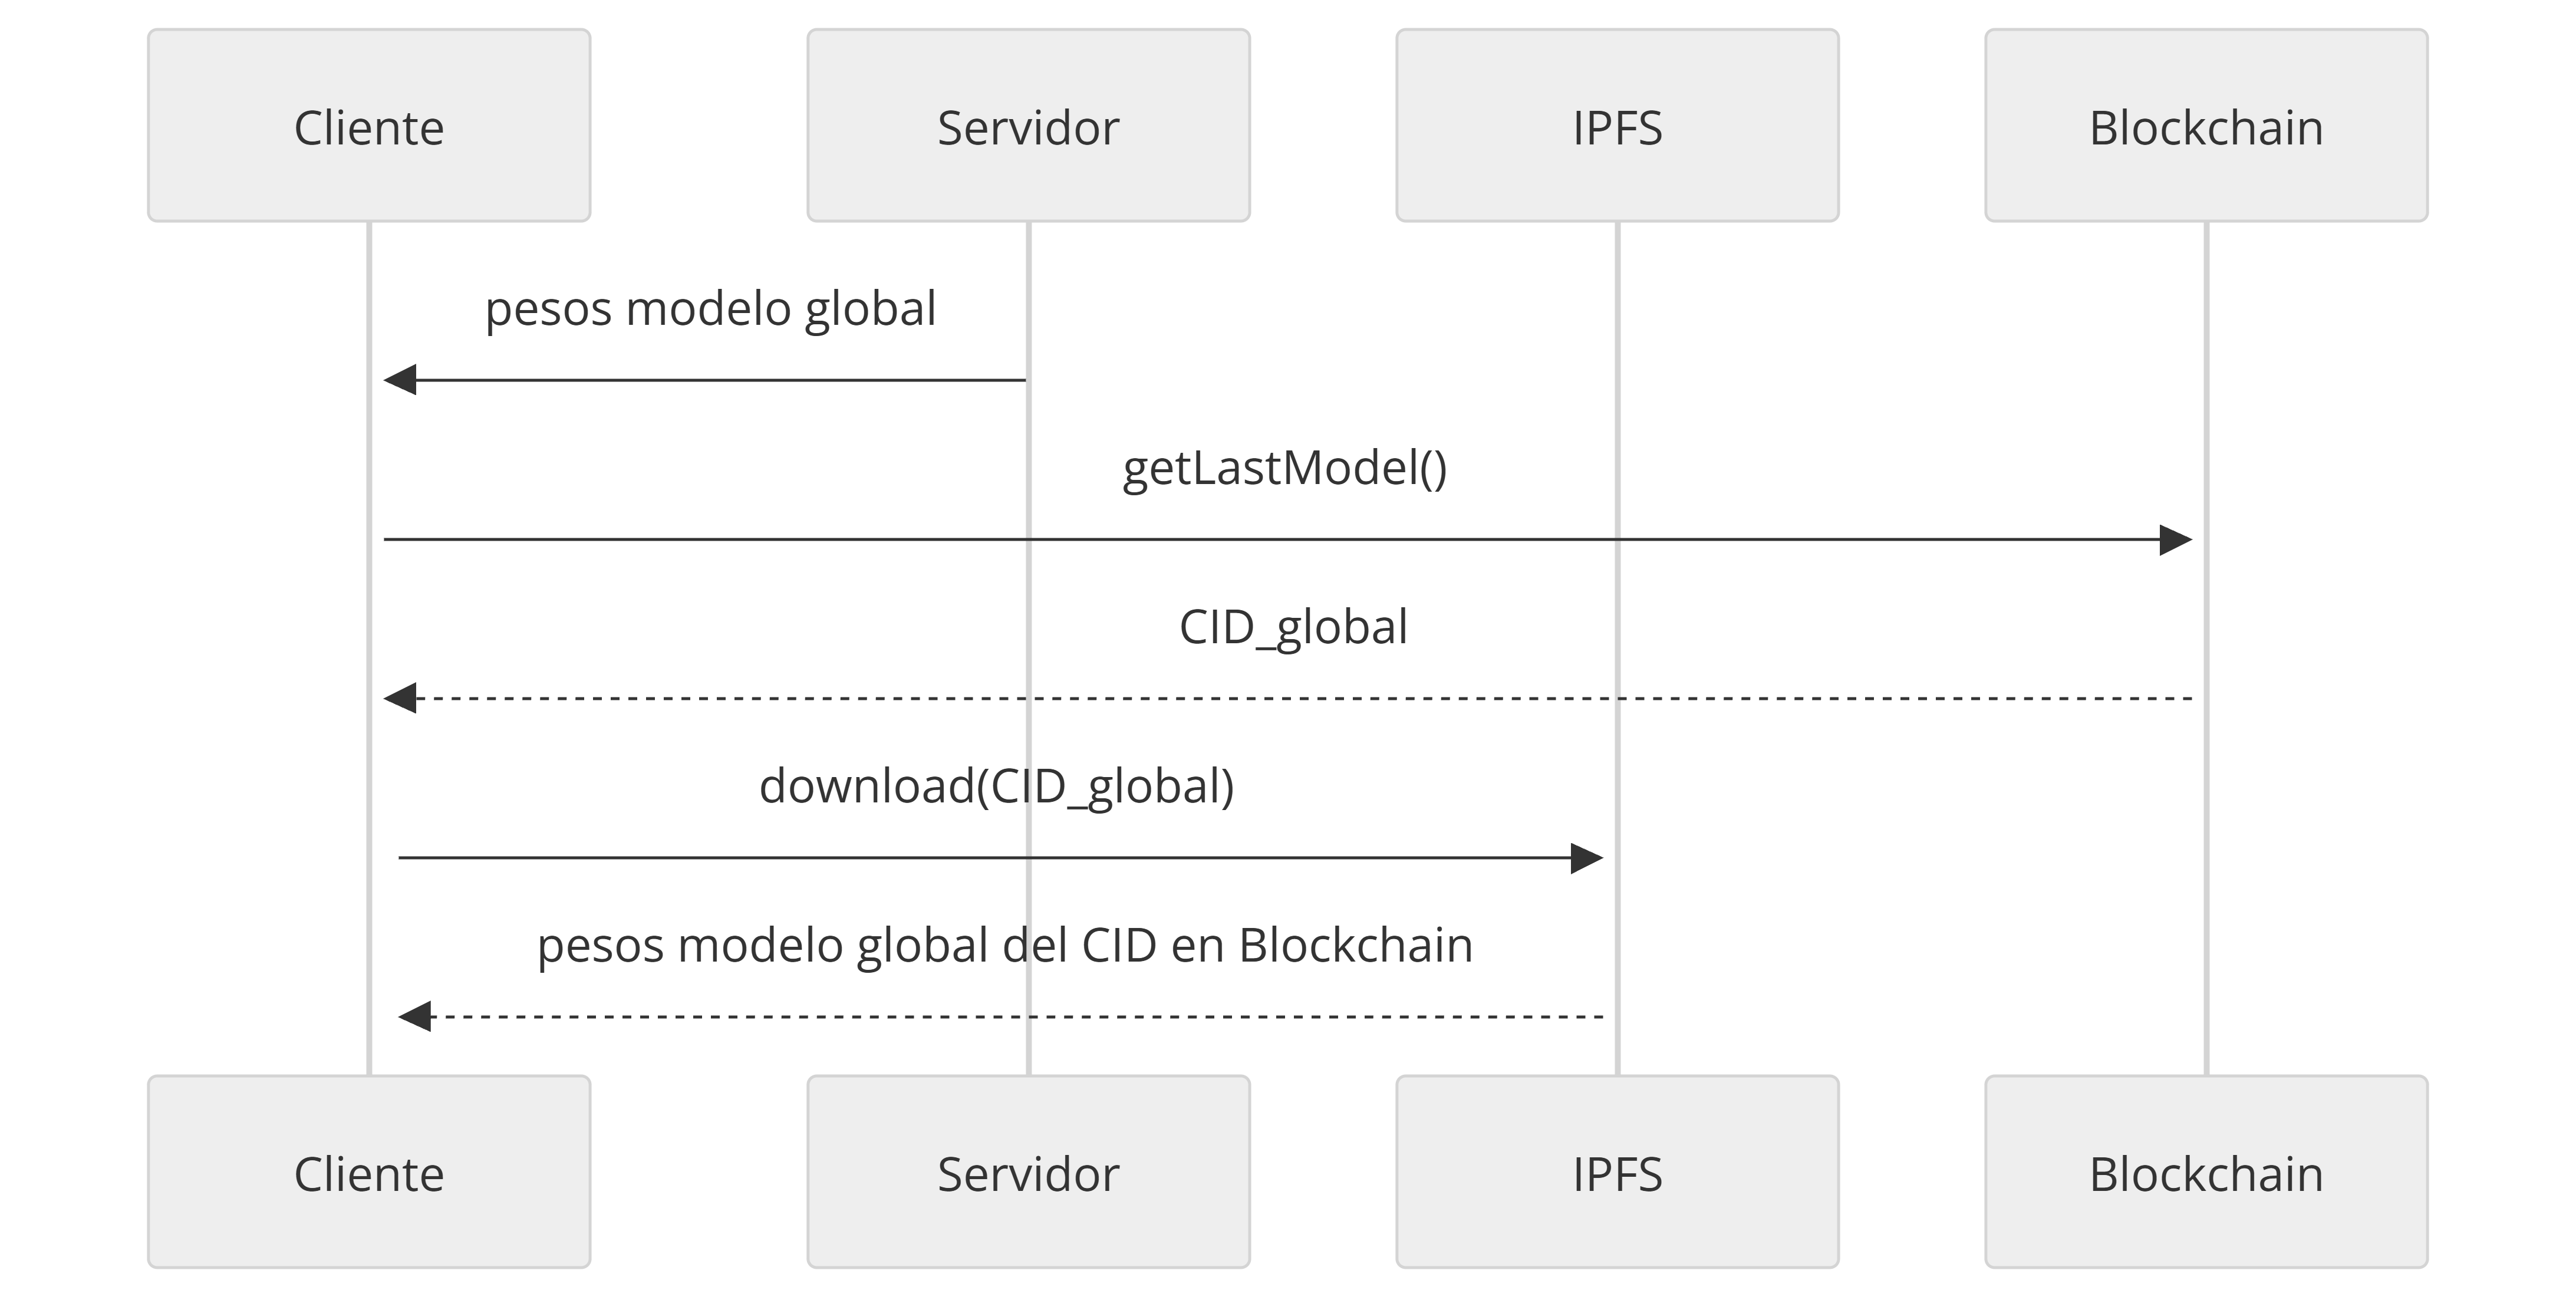
\includegraphics[width=\columnwidth]{figuras/inicio_ronda_good.png}
    \caption{Fase 1: Verificación descendente en el cliente: cotejo del modelo recibido frente al CID registrado on-chain y descargado de IPFS.}
    \label{fig:flujo_cliente_verif}
\end{figure}

\subsubsection{Fase 2: Entrenamiento Local y Registro de Contribución}
Si la comprobación previa es satisfactoria (Figura~\ref{fig:flujo_cliente_entreno}):
\begin{enumerate}
    \item El cliente ejecuta el entrenamiento local con su partición privada de datos.
    \item Serializa los nuevos pesos locales $w_k^{(t)}$ y los almacena en IPFS, obteniendo $\text{CID}_k^{(t)}$.
    \item Emite una transacción firmada con su clave privada invocando \texttt{registerClientModel(}$t$, $\text{CID}_k^{(t)}$\texttt{)} y aguarda el recibo (\textit{receipt}) de inclusión en el bloque IBFT 2.0.
    \item Retorna a Flower los parámetros junto con el identificador $\text{CID}_k^{(t)}$ y su clave pública.
\end{enumerate}

\begin{figure}[H]
    \centering
    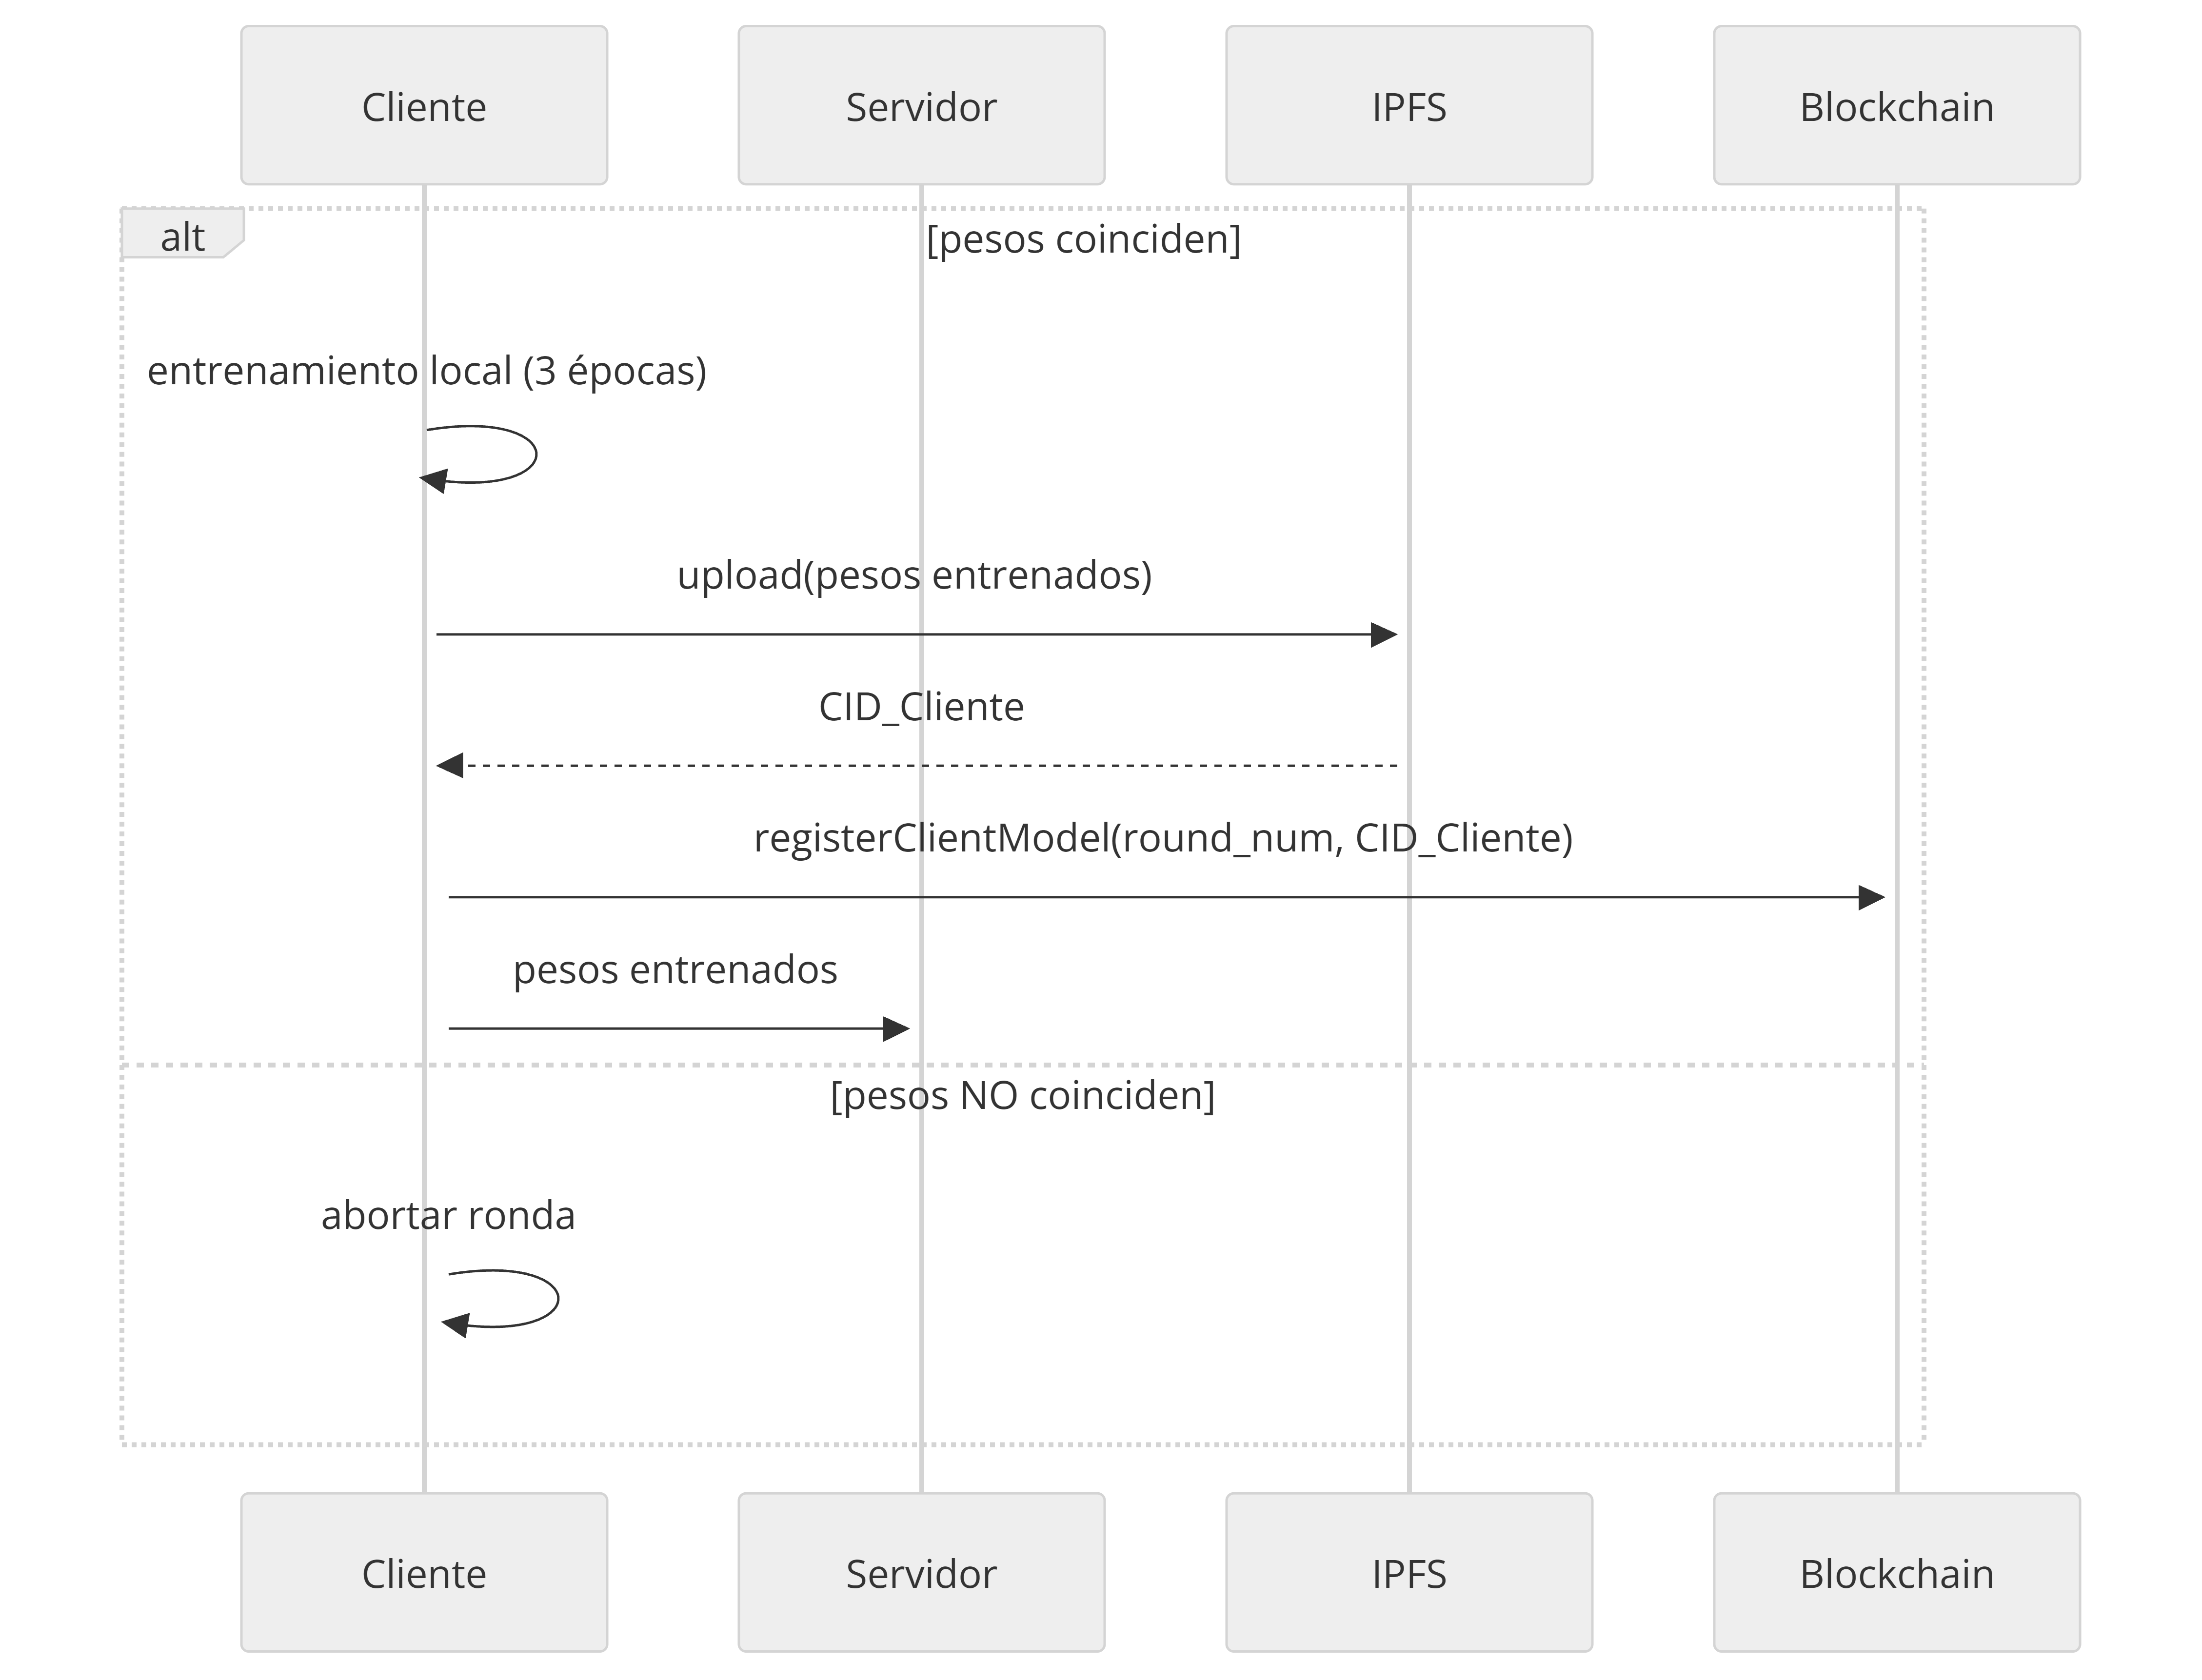
\includegraphics[width=\columnwidth]{figuras/entrenamiento.png}
    \caption{Fase 2: Entrenamiento local en el cliente, subida de pesos a IPFS y transacción firmada a Hyperledger Besu.}
    \label{fig:flujo_cliente_entreno}
\end{figure}

\subsubsection{Fase 3: Verificación Ascendente y Agregación Global}
Al recibir los pesos de los clientes en el servidor agregador (Figura~\ref{fig:flujo_servidor_agregacion}):
\begin{enumerate}
    \item Para cada cliente $k$, el servidor consulta \texttt{getClientModel(}$t$, $\text{address}_k$\texttt{)} en la Blockchain.
    \item Comprueba que el CID reportado por gRPC coincida con el hash inmutable registrado y firmado por el cliente. Si la comprobación falla, la contribución es descartada de forma preventiva.
    \item Aplica la agregación ponderada FedAvg únicamente sobre las contribuciones debidamente auditadas:
    \begin{equation}
    w^{(t+1)} = \sum_{k \in \mathcal{K}_{valid}} \frac{n_k}{n_{valid}} \, w_k^{(t)}
    \end{equation}
    \item Sube el nuevo modelo consolidado a IPFS, obteniendo $\text{CID}_{global}^{(t+1)}$, y lo sella en Besu invocando \texttt{updateModel(}$t+1$, $\text{CID}_{global}^{(t+1)}$\texttt{)}.
\end{enumerate}

\begin{figure}[H]
    \centering
    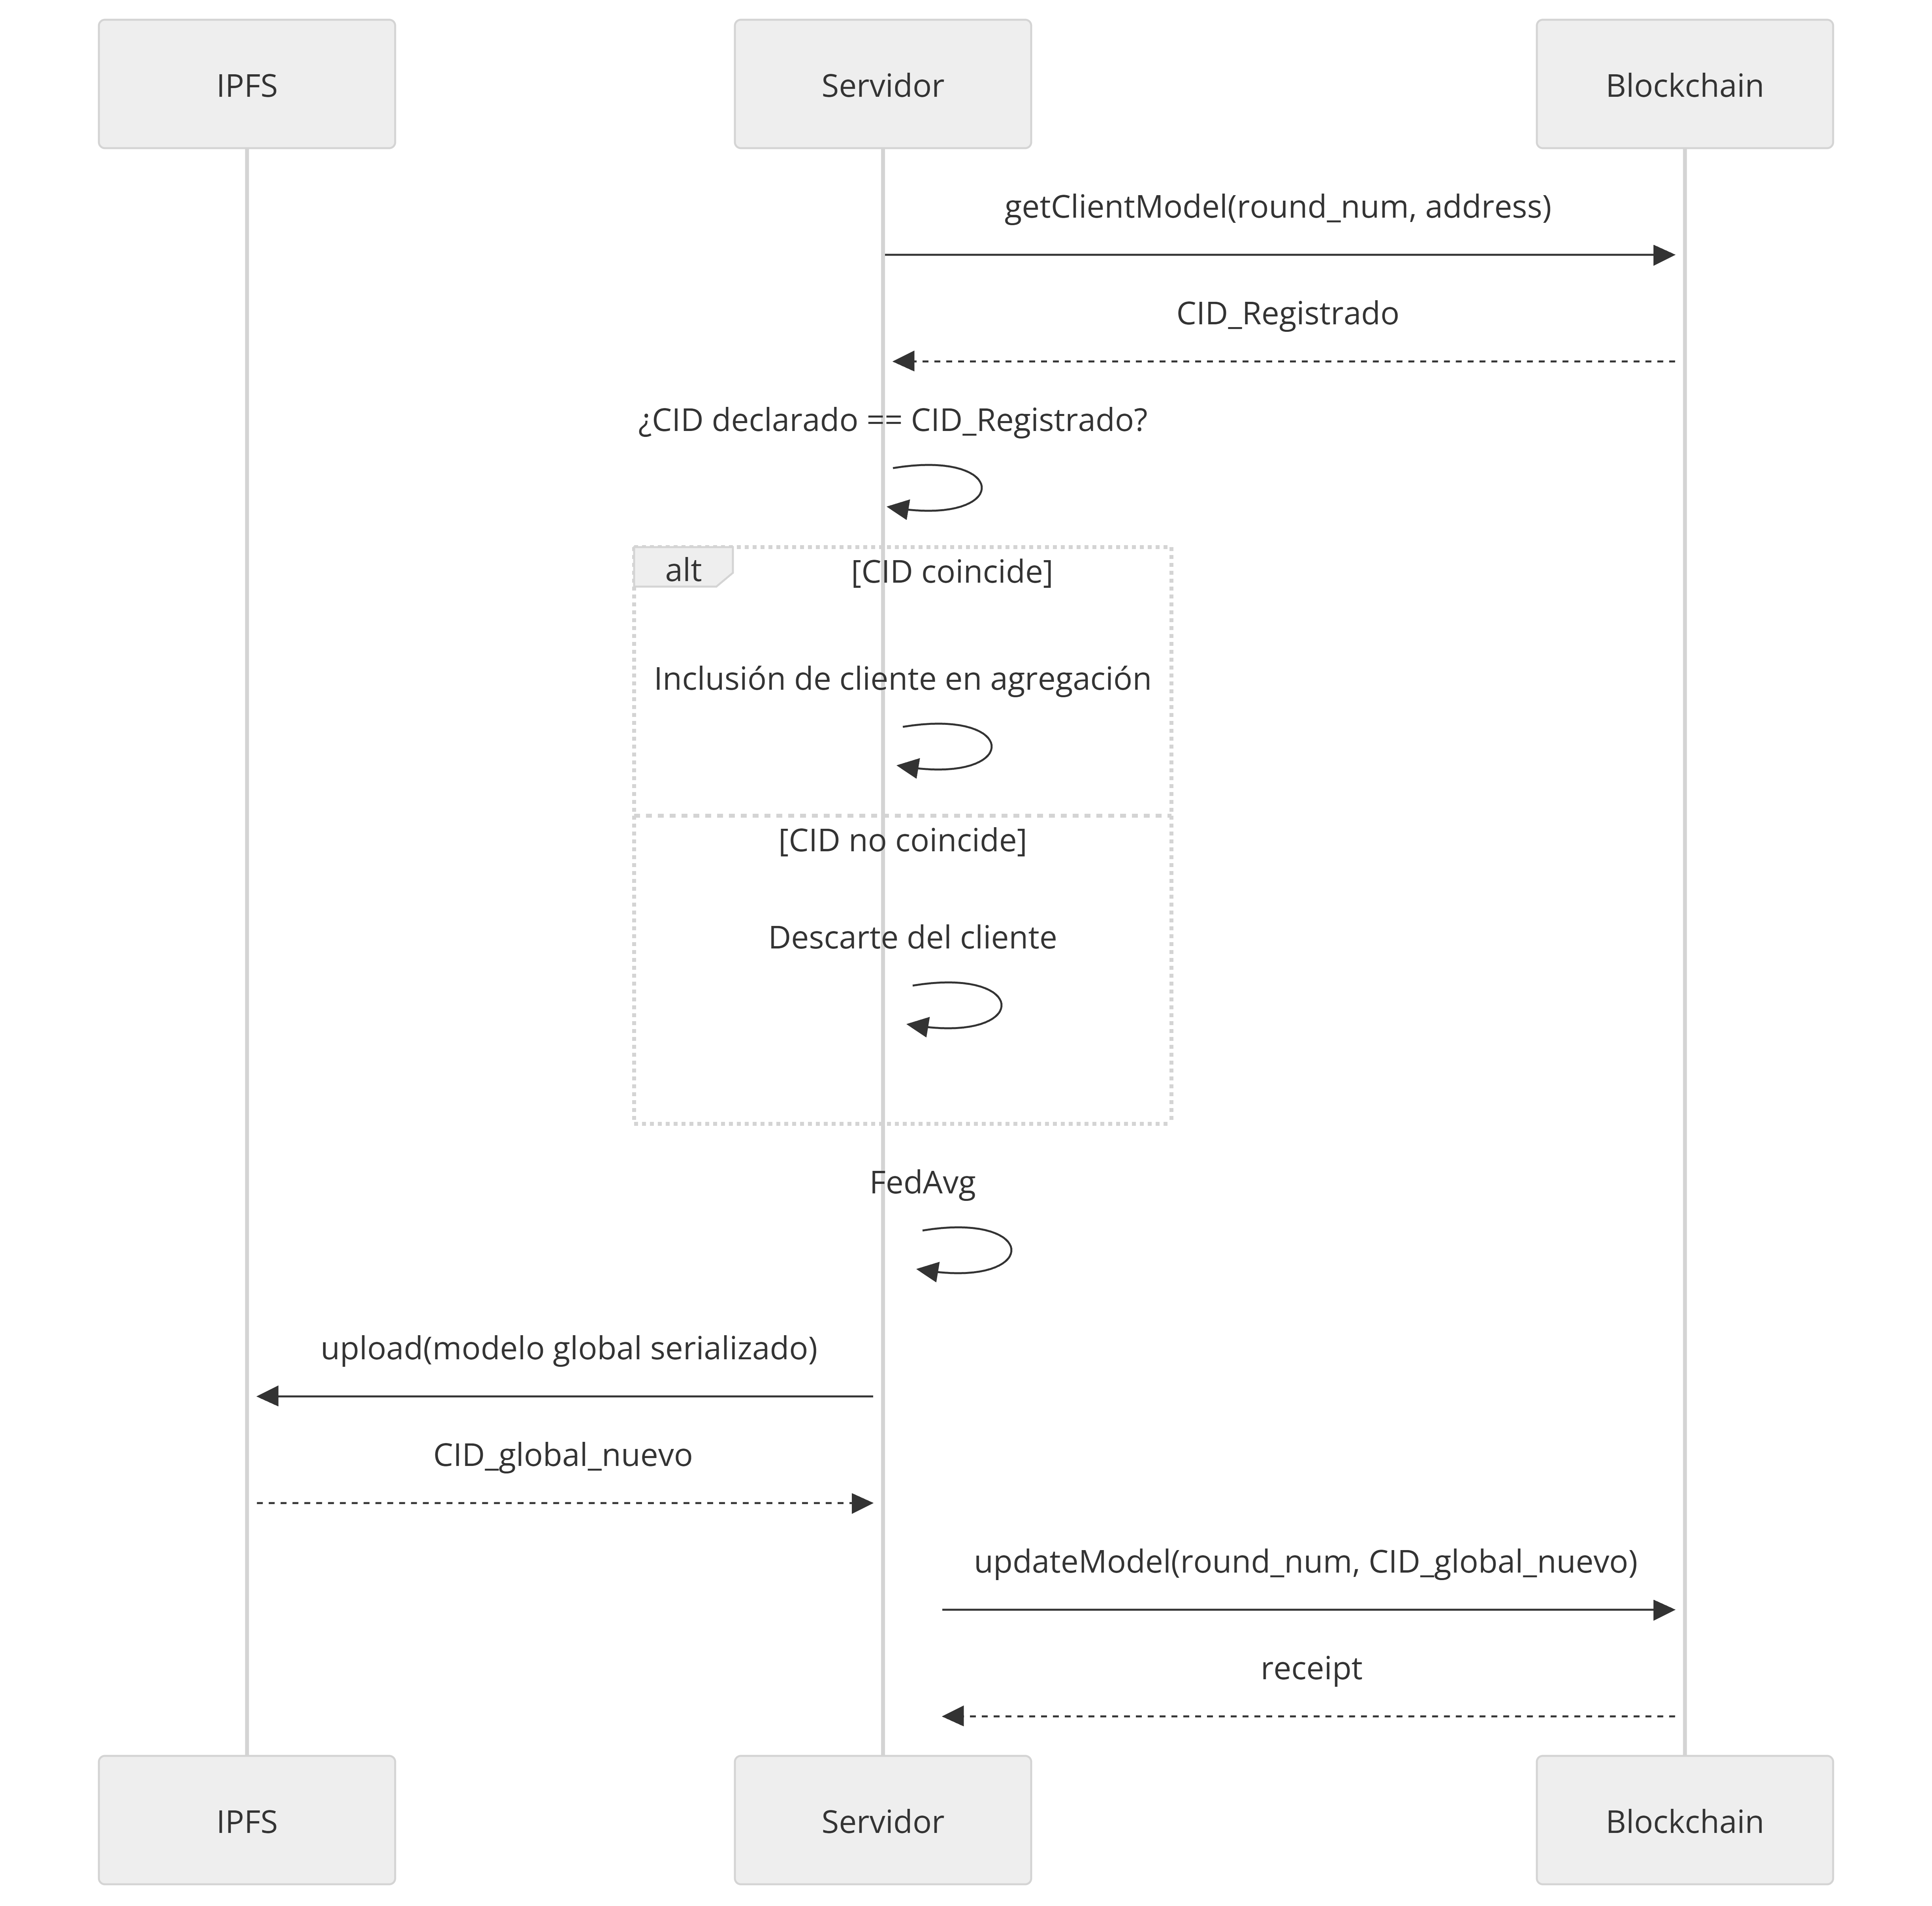
\includegraphics[width=\columnwidth]{figuras/fin_ronda.png}
    \caption{Fase 3: Verificación ascendente en el servidor: validación de CIDs on-chain, agregación FedAvg y sellado global de ronda.}
    \label{fig:flujo_servidor_agregacion}
\end{figure}

Este mecanismo garantiza trazabilidad completa de extremo a extremo, no repudio y aislamiento de participantes disidentes.

% !TeX root = ../main.tex
\section{Implementación y Entorno Experimental}
\label{sec:implementacion}

Con el fin de aislar y evaluar cuantitativamente el sobrecoste introducido por la capa de trazabilidad y auditoría, se desplegó un banco de pruebas experimental representativo de un entorno de computación distribuida vehicular.

\subsection{Infraestructura de Hardware y Software}
La evaluación empírica se llevó a cabo utilizando dos estaciones físicas interconectadas en la misma red de área local (LAN), cuyas especificaciones técnicas se detallan en la Tabla~\ref{tab:testbed_hardware}:
\begin{itemize}
    \item \textbf{Estación 1 (Nodo Central)}: Aloja el servidor agregador Flower, el nodo RPC principal de la red Besu y el nodo de almacenamiento IPFS.
    \item \textbf{Estación 2 (Nodos de Borde / Clientes)}: Aloja y ejecuta los clientes de entrenamiento federado (\textit{members} 2 y 3).
\end{itemize}

\begin{table}[H]
\centering
\caption{Especificaciones del banco de pruebas experimental.}
\label{tab:testbed_hardware}
\resizebox{\columnwidth}{!}{%
\begin{tabular}{lll}
\toprule
\textbf{Parámetro} & \textbf{Estación 1 (Servidor/RPC)} & \textbf{Estación 2 (Clientes)} \\
\midrule
Procesador & Intel Core i5-1135G7 & Intel Core i7-9700 \\
Frecuencia base & 2,40 GHz & 3,00 GHz \\
Núcleos / Hilos & 4 núcleos / 8 hilos & 8 núcleos / 8 hilos \\
Memoria RAM & 7,6 GB (asignada en WSL2) & 8,0 GB \\
Sistema Operativo & Ubuntu 22.04 LTS (WSL2) & Windows 11 \\
\bottomrule
\end{tabular}%
}
\end{table}

El stack de software está compuesto por Hyperledger Besu con soporte de transacciones privadas mediante Tessera, orquestado mediante Docker Compose; el daemon IPFS Kubo (\texttt{v0.32.1}); Python \texttt{3.12} con PyTorch para la inferencia y optimización neuronal; Flower (\texttt{flwr}) para la coordinación gRPC de la federación; y la biblioteca \texttt{web3.py} para la conectividad JSON-RPC con la EVM.
\\

Las dos estaciones se encuentran comunicadas a través de un enlace de red de área local inalámbrico (Wi-Fi 802.11ac a 5~GHz), registrando una latencia media de ida y vuelta (\textit{RTT ping}) de $3{,}8 \pm 1{,}1$~ms y un ancho de banda sostenido de 100~Mbps. El tamaño del modelo neuronal serializado (\texttt{NetCliente}) es de exactamente $1{,}95$~MB en formato binario. Para garantizar un rendimiento óptimo en la capa de almacenamiento distribuido, la subida a IPFS se efectúa mediante la API HTTP en el endpoint \texttt{/api/v0/add?pin=false}, lo que permite registrar y generar el identificador CID en memoria local en milisegundos.

\subsection{Modelo Neuronal y Conjunto de Datos Vehicular}
Como caso de uso para simular un sistema de asistencia a la conducción en vehículos conectados y autónomos (CAV), se adoptó el dataset de clasificación de eventos de tráfico del grupo CloudLab-AIA~\cite{cloudlabaia_flblockchain}. 
\\

El problema consiste en una tarea de clasificación multiclase orientada a la detección en carretera con cuatro categorías:
\begin{enumerate}
    \item Accidente vial (\texttt{accident}).
    \item Congestión o tráfico denso (\texttt{dense\_traffic}).
    \item Condiciones meteorológicas adversas (\texttt{meteorology}).
    \item Flujo de tráfico fluido (\texttt{sparse\_traffic}).
\end{enumerate}

El conjunto de datos comprende un total de 3.415 imágenes distribuidas en: meteorología adversa (1.027), tráfico fluido (947), tráfico denso (778) y accidentes (663). Las imágenes se preprocesan mediante reescalado a una resolución de $32 \times 32$ píxeles en tres canales cromáticos (RGB) y normalización estándar. Para preservar la comparabilidad estadística y eliminar sesgos de distribución, el conjunto de datos se reparte entre los $K=2$ clientes según un esquema independiente e idénticamente distribuido (IID).
\\

El modelo implementado (\texttt{NetCliente}) es una red neuronal convolucional (CNN) estructurada en dos bloques convolucionales consecutivos (con kernels de $3 \times 3$, función de activación ReLU y submuestreo por \textit{Max Pooling}), seguidos de dos capas densas completamente conectadas (\textit{fully connected}) que proyectan el vector de características hacia las 4 neuronas de salida. El entrenamiento se realiza mediante la función de pérdida de entropía cruzada (\textit{Cross-Entropy Loss}) y el algoritmo de optimización Adam con una tasa de aprendizaje $\eta = 10^{-3}$, configurando un tamaño de lote (\textit{batch size}) de 16 muestras en entrenamiento y 32 en evaluación, 3 épocas locales de entrenamiento por ronda y un horizonte total de 30 rondas federadas.
\\

Es importante remarcar que el propósito primordial de este estudio no radica en diseñar el modelo más óptimo ni en maximizar su precisión de clasificación, sino en utilizar la arquitectura de aprendizaje federado como un banco de pruebas realista para generar y analizar métricas cuantitativas del sistema (sobrecoste temporal, escalabilidad y consumo de gas). La optimización del modelo (ajuste de hiperparámetros, mitigación del sobreajuste o empleo de arquitecturas más profundas) se plantea deliberadamente como trabajo futuro, actuando aquí la red neuronal como una carga de trabajo experimental de referencia.

\subsection{Matriz de Configuraciones Experimentales}
Para desglosar y desacoplar de forma analítica el impacto individual de cada componente, se diseñaron cinco configuraciones experimentales (E1 a E5), resumidas en la Tabla~\ref{tab:configuraciones}.

\begin{table}[H]
\centering
\caption{Matriz de configuraciones experimentales evaluadas.}
\label{tab:configuraciones}
\resizebox{\columnwidth}{!}{%
\begin{tabular}{ccccc}
\toprule
\textbf{ID Exp.} & \textbf{Estaciones} & \textbf{Capa Blockchain} & \textbf{Validadores} & \textbf{Objetivo} \\
\midrule
E1 & 1 & Sí & 4 & Sobrecarga BC local \\
E2 & 1 & No & --- & Baseline local \\
E3 & 2 & No & --- & Baseline distribuido \\
E4 & 2 & Sí & 4 & Sobrecarga BC distribuida \\
E5 & 2 & Sí & 7 & Escalabilidad IBFT 2.0 \\
\bottomrule
\end{tabular}%
}
\end{table}

Este diseño metodológico permite efectuar comparaciones controladas de una sola variable:
\begin{itemize}
    \item \textbf{Coste directo de Blockchain}: Comparación de E1 vs. E2 en entorno monomáquina, y de E4 vs. E3 en entorno distribuido en red.
    \item \textbf{Efecto de la distribución física}: Comparación de E2 vs. E3 (sin Blockchain) y de E1 vs. E4 (con Blockchain de 4 validadores).
    \item \textbf{Escalado del consenso BFT}: Comparación de E4 (4 validadores) vs. E5 (7 validadores), evaluando la penalización de latencia al elevar la tolerancia a fallos de $f=1$ a $f=2$.
\end{itemize}


% !TeX root = ../main.tex
\section{Evaluación Experimental y Resultados}
\label{sec:evaluacion}

En esta sección se analiza cuantitativamente el comportamiento del sistema a lo largo de las 30 rondas de entrenamiento federado, respondiendo a las preguntas de investigación formuladas: el sobrecoste temporal de la capa de auditoría, el comportamiento ante el escalado físico y de consenso, y el consumo de gas en la EVM.

\subsection{Convergencia del Modelo y Análisis de Pérdida}
La Figura~\ref{fig:convergencia} ilustra la evolución de la función de pérdida de entropía cruzada en el conjunto de validación durante las 30 iteraciones federadas.

\begin{figure}[H]
    \centering
    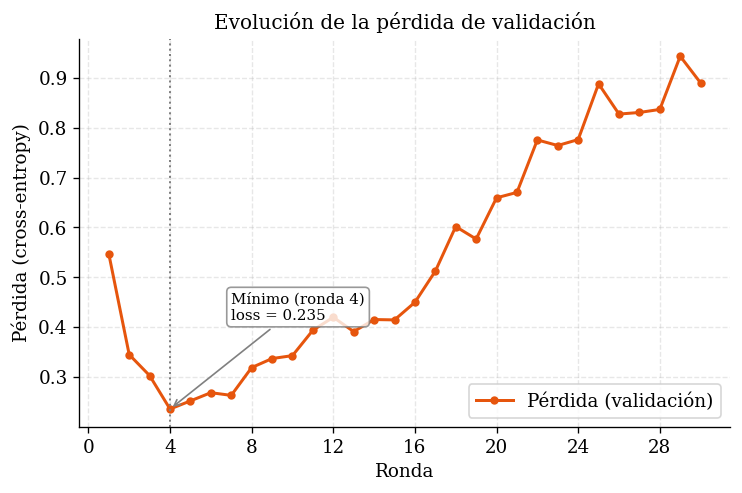
\includegraphics[width=\columnwidth]{figuras/convergencia_loss.png}
    \caption{Evolución de la pérdida de validación (\textit{cross-entropy}) a lo largo de las 30 rondas federadas.}
    \label{fig:convergencia}
\end{figure}

El modelo muestra un rápido aprendizaje inicial, alcanzando un mínimo de pérdida óptimo en la ronda 4 ($\mathcal{L} \approx 0{,}24$) con una precisión de clasificación que se estabiliza en el $97\%$. A partir de dicho punto, la pérdida experimenta un incremento gradual y sostenido hasta situarse en torno a $0{,}90$ hacia el final del ciclo. Este comportamiento representa un caso paradigmático de sobreajuste (\textit{overfitting}) provocado por el régimen de 90 épocas acumuladas (3 épocas locales $\times$ 30 rondas federadas) sobre un conjunto de entrenamiento acotado, donde la red incrementa excesivamente su confianza en predicciones.

El mínimo de pérdida en la ronda 4 sugiere que la incorporación de técnicas como la parada temprana (\textit{early stopping}) habría detenido el entrenamiento en ese instante, logrando una versión más ajustada del clasificador. Sin embargo, se mantuvieron de forma deliberada las 30 rondas predefinidas porque el objetivo central de esta investigación no es optimizar el modelo de IA ni perseguir su punto de máxima eficiencia, sino someter la infraestructura de aprendizaje federado a una carga constante para extraer métricas cuantitativas reproducibles (latencia por ronda, tiempo de confirmación y coste de gas). De este modo, la optimización fina del modelo se pospone como trabajo futuro.

Es fundamental enfatizar que \textbf{la curva de convergencia es estrictamente idéntica con o sin la presencia de Blockchain}. Dado que la capa de trazabilidad opera exclusivamente en la verificación e indexación criptográfica fuera de cadena y no interfiere en los tensores ni en los gradientes de FedAvg, la dinámica de entrenamiento se mantiene inalterada.

\subsection{Visión General del Rendimiento Temporal}
La Tabla~\ref{tab:tiempos_resumen} sintetiza el tiempo total requerido por ronda federada en las cinco configuraciones, reportando la mediana, media y desviación típica. Asimismo, la Figura~\ref{fig:tiempo_todas} refleja la serie temporal a lo largo de las 30 rondas.
\\

En la configuración distribuida E4 se registró una desviación típica notablemente superior (12,63 s) debida a un pico transitorio en la ronda 7 (121,3 s). Un análisis de rango intercuartílico confirmó que este valor anómalo obedeció a contención momentánea de memoria en el subsistema de virtualización WSL2. En consecuencia, se adopta la \textbf{mediana} como métrica central de referencia por su robustez frente a fluctuaciones esporádicas del entorno operativo.

\begin{table}[H]
\centering
\caption{Tiempo total de ejecución por ronda federada en cada configuración.}
\label{tab:tiempos_resumen}
\resizebox{\columnwidth}{!}{%
\begin{tabular}{cccccc}
\toprule
\textbf{Exp.} & \textbf{Máq.} & \textbf{Configuración} & \textbf{Mediana (s)} & \textbf{Media (s)} & \textbf{Desv. (s)} \\
\midrule
E1 & 1 & 4 val · con BC & 89,37 & 91,84 & 6,34 \\
E2 & 1 & Baseline sin BC & 84,15 & 82,18 & 6,95 \\
E3 & 2 & Baseline sin BC & 64,26 & 64,27 & 0,74 \\
E4 & 2 & 4 val · con BC & 71,29 & 77,05 & 12,63 \\
E5 & 2 & 7 val · con BC & 70,88 & 73,40 & 4,71 \\
\bottomrule
\end{tabular}%
}
\end{table}

\begin{figure}[H]
    \centering
    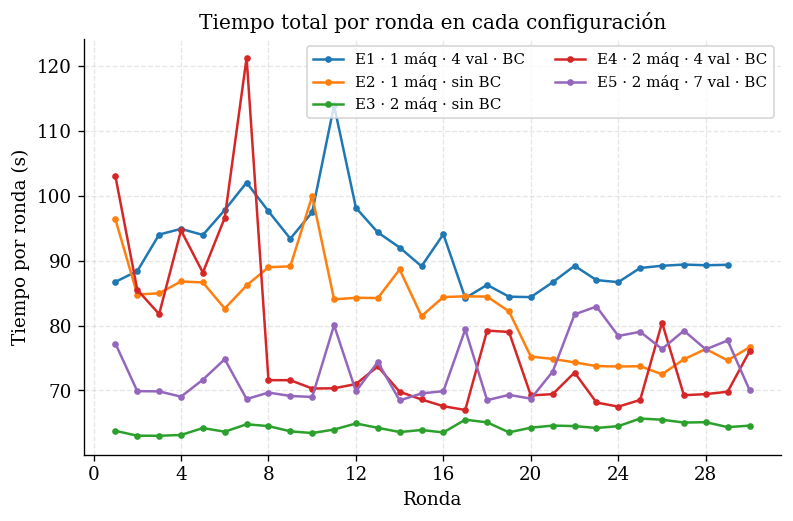
\includegraphics[width=\columnwidth]{figuras/tiempo_ronda_todas.png}
    \caption{Comparativa del tiempo total por ronda federada en las cinco configuraciones experimentales.}
    \label{fig:tiempo_todas}
\end{figure}

\subsection{Sobrecoste Temporal de la Capa Blockchain}
Para aislar el coste intrínseco impuesto por las llamadas a IPFS, las transacciones a la EVM y la sincronización con Besu, se comparan configuraciones que difieren únicamente en la inclusión de la Blockchain (Figura~\ref{fig:coste_bc}):
\begin{itemize}
    \item \textbf{Escenario Monomáquina (E1 vs. E2)}: El tiempo mediano pasa de 84,15 s a 89,37 s, lo que representa un sobrecoste de tan solo \textbf{5,22 s (+6,2\%)}.
    \item \textbf{Escenario Distribuido (E4 vs. E3)}: El tiempo mediano aumenta de 64,26 s a 71,29 s, suponiendo una sobrecarga de \textbf{7,03 s (+10,9\%)}.
\end{itemize}

\begin{figure}[H]
    \centering
    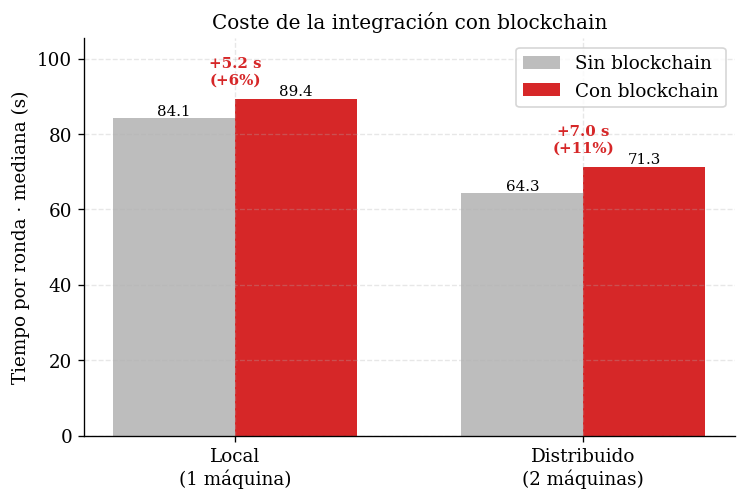
\includegraphics[width=\columnwidth]{figuras/coste_blockchain.png}
    \caption{Sobrecoste temporal inducido por la integración de la Blockchain en entornos local y distribuido.}
    \label{fig:coste_bc}
\end{figure}

Este incremento marginal ($\sim$5 a 7 segundos por ciclo) engloba la serialización con \texttt{pickle}, la publicación en IPFS, la firma ECDSA, la confirmación del bloque IBFT 2.0 y la verificación cruzada en cliente y servidor. Para sistemas que requieren auditoría legal o certificación de integridad, asumir un 10\% de penalización temporal constituye una penalización sumamente ventajosa.

\subsection{Efecto de la Distribución Física y Contención de Recursos}
La comparación entre una estación y dos estaciones revela un hallazgo crítico (Figura~\ref{fig:coste_dist}): distribuir los nodos en la red local \textbf{reduce drásticamente el tiempo de ronda}, tanto sin Blockchain (de 84,15 s a 64,26 s; una reducción de -23,6\%) como con Blockchain (de 89,37 s a 71,29 s; una reducción de -20,2\%).

\begin{figure}[H]
    \centering
    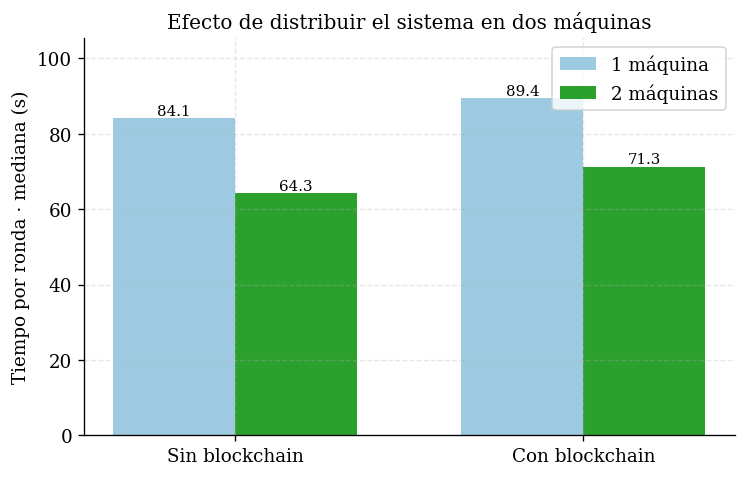
\includegraphics[width=\columnwidth]{figuras/coste_distribucion.png}
    \caption{Efecto de la distribución física de nodos sobre el tiempo de ciclo: mitigación de cuellos de botella de CPU/memoria.}
    \label{fig:coste_dist}
\end{figure}

La explicación reside en la eliminación de la contención de recursos. En la configuración local monomáquina, el daemon de Besu, los contenedores de validadores, IPFS y los procesos PyTorch compiten por los mismos 8 hilos y 7,6 GB de RAM. Al delegar la computación de los clientes a la Estación 2, la ganancia en capacidad de cómputo paralelo supera ampliamente la ligera latencia añadida por la transmisión de paquetes en la red inalámbrica.

\subsection{Impacto del Escalado de Validadores y Consenso IBFT 2.0}
Al comparar E4 (4 validadores) con E5 (7 validadores), el tiempo total de ronda se mantiene virtualmente indistinguible (71,29 s frente a 70,88 s). Esto confirma que el tiempo dominante en una ronda federada es la optimización neuronal local de los clientes, y no la latencia del bloque.

\begin{figure}[H]
    \centering
    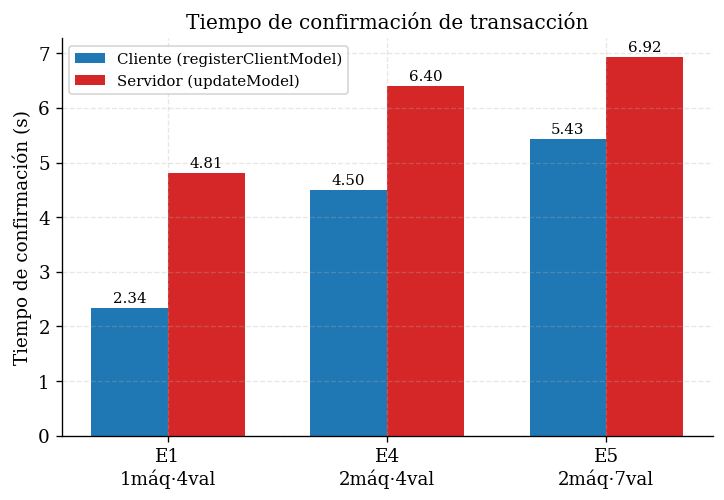
\includegraphics[width=\columnwidth]{figuras/tiempo_confirmacion.png}
    \caption{Tiempo medio de confirmación de transacción según topología y número de validadores en Hyperledger Besu.}
    \label{fig:tiempo_confirmacion}
\end{figure}

No obstante, al desagregar específicamente el \textbf{tiempo de confirmación de transacciones} (Figura~\ref{fig:tiempo_confirmacion}), el comportamiento del protocolo IBFT 2.0 se manifiesta nítidamente:
\begin{itemize}
    \item Para la transacción del cliente (\texttt{registerClientModel}), la latencia de confirmación crece de 4,50 s (con 4 validadores) a 5,43 s (con 7 validadores).
    \item Para la transacción del servidor (\texttt{updateModel}), el tiempo se eleva de 6,40 s a 6,92 s.
\end{itemize}
Este incremento lineal obedece a las fases de intercambio de mensajes (\textit{Prepare} y \textit{Commit}) del protocolo IBFT 2.0, que exige recabar firmas del quórum de supermayoría ($2f+1$). Sin embargo, este sobrecoste queda totalmente diluido en el tiempo total del entrenamiento, demostrando que elevar la tolerancia a fallos de $f=1$ a $f=2$ es viable sin penalizar el rendimiento macroscópico del sistema.

\subsection{Consumo y Previsibilidad del Gas en la EVM}
La Figura~\ref{fig:consumo_gas} ilustra el consumo de gas computacional de las operaciones registradas a lo largo de las rondas.

\begin{figure}[H]
    \centering
    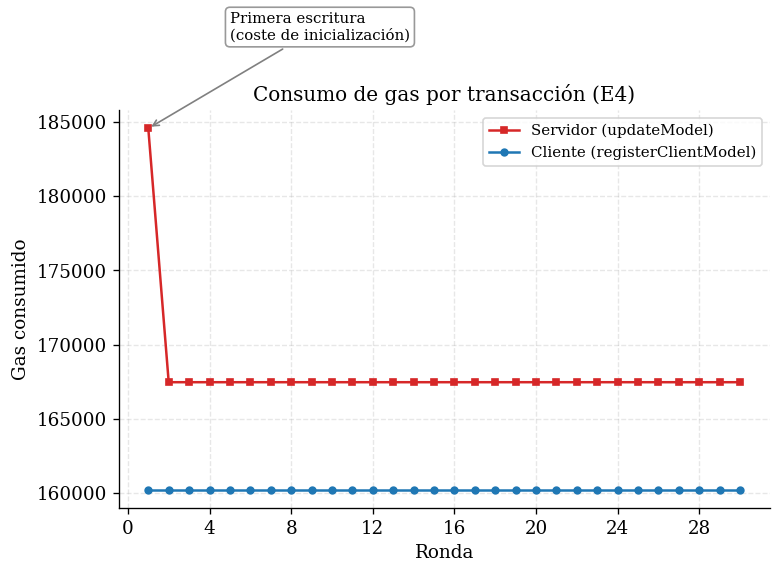
\includegraphics[width=\columnwidth]{figuras/consumo_gas.png}
    \caption{Consumo de gas en la Máquina Virtual de Ethereum por tipo de transacción a lo largo de las 30 rondas.}
    \label{fig:consumo_gas}
\end{figure}

El perfil de consumo resulta rigurosamente constante en todas las iteraciones subsiguientes:
\begin{itemize}
    \item \texttt{registerClientModel}: exactamente \textbf{160.200 unidades de gas}.
    \item \texttt{updateModel}: exactamente \textbf{167.460 unidades de gas}.
\end{itemize}
La única excepción observable corresponde a la ronda 0 del servidor, que demandó \textbf{184.560 unidades de gas}. Dicha discrepancia (+17.100 unidades) responde al coste intrínseco de la instrucción \texttt{SSTORE} de la EVM al escribir por primera vez en posiciones de memoria previamente vacías (\textit{cold write}) y modificar el valor del flag booleano \texttt{hasModel}.
\\

La invariabilidad del consumo valida formalmente el diseño desacoplado: al mantener almacenamiento de complejidad $\mathcal{O}(1)$ en el contrato (hashes y metadatos acotados), el coste en recursos computacionales es determinista e independiente del tamaño del modelo neuronal o del número de rondas ejecutadas.


% !TeX root = ../main.tex
\section{Conclusiones y Trabajo Futuro}
\label{sec:conclusiones}

En este artículo se ha presentado, implementado y validado experimentalmente un marco integral para garantizar la trazabilidad, integridad y auditoría criptográfica en sistemas de Aprendizaje Federado, combinando una red Blockchain permisionada (Hyperledger Besu) con almacenamiento direccionable fuera de cadena (IPFS) y el framework Flower.

\subsection{Conclusiones Principales}
Los resultados obtenidos permiten extraer las siguientes conclusiones clave:
\begin{itemize}
    \item \textbf{Viabilidad técnica y sobrecoste temporal asumible}: La integración de la capa de trazabilidad introduce una penalización de ciclo de únicamente entre el \textbf{6,2\%} (en entorno local) y el \textbf{10,9\%} (en entorno distribuido en red), equivalente a entre 5 y 7 segundos por ronda federada. Este sobrecoste responde afirmativamente al dilema de rendimiento vs. seguridad, demostrando que la auditabilidad de extremo a extremo es plenamente asumible en sistemas de IA distribuida.
    \item \textbf{Eficacia de la doble verificación cruzada}: El diseño propuesto erradica la dependencia de un servidor central como punto único de confianza. Mediante el cotejo automático de CIDs de IPFS frente a los registros inmutables on-chain, los clientes quedan protegidos frente a modelos globales corruptos, mientras que el agregador descarta de inmediato contribuciones disidentes no firmadas.
    \item \textbf{Eficiencia y predictibilidad on-chain}: El desacoplamiento arquitectónico mediante IPFS asegura un consumo de gas estrictamente determinista y de complejidad $\mathcal{O}(1)$ ($\sim$160.200 gas para clientes y $\sim$167.460 gas para el servidor), evitando cualquier saturación del estado de la EVM con independencia del tamaño de los modelos.
    \item \textbf{Escalabilidad del consenso BFT}: Incrementar los nodos validadores de 4 a 7 (duplicando la tolerancia a fallos bizantinos de $f=1$ a $f=2$) apenas eleva la latencia de confirmación en $\sim$0,9 segundos, quedando este incremento absorbido de forma imperceptible dentro del tiempo global de entrenamiento local.
\end{itemize}

\subsection{Limitaciones y Trabajo Futuro}
Como líneas de desarrollo futuro que amplían el alcance de este trabajo, se plantean:
\begin{enumerate}
    \item \textbf{Optimización y regularización del modelo de IA}: Dado que la meta primordial de este artículo consistió en evaluar la infraestructura y extraer métricas cuantitativas del sistema FL-Blockchain, la optimización fina de la red neuronal quedó fuera del alcance primario. Como línea futura se contempla incorporar criterios de parada temprana (\textit{early stopping}), técnicas de regularización (Dropout, normalización de batches) y arquitecturas convolucionales avanzadas para maximizar la generalización.
    \item \textbf{Mecanismos de reputación y penalización on-chain}: Explotar el historial inmutable de contribuciones para articular algoritmos de puntuación de clientes o penalización (\textit{slashing}) económica/lógica de nodos maliciosos recurrentes.
    \item \textbf{Agregación bizantina avanzada}: Complementar el esquema con estrategias de agregación robustas frente a envenenamiento no evidente (como Krum o Trimmed Mean) coordinadas desde el propio contrato.
    \item \textbf{Entornos no-IID y despliegue vehicular V2X}: Evaluar la robustez del framework bajo distribuciones de datos altamente heterogéneas y desplegar nodos en hardware embarcado (\textit{edge computing}, como NVIDIA Jetson) con conectividad celular 5G/V2X.
    \item \textbf{Gestión criptográfica de claves}: Sustituir el esquema de cuentas actual por módulos de seguridad de hardware (HSM) o almacenes seguros de secretos tipo Key Vault para un despliegue conforme a estándares industriales.
\end{enumerate}
En síntesis, la arquitectura validada demuestra que la convergencia entre Blockchain y Aprendizaje Federado no solo es factible, sino que constituye una solución sólida y escalable para el despliegue confiable de inteligencia artificial en entornos críticos y cooperativos.



\bibliography{bibliografia}

\end{document}
